% Fig. 2.10 / spec Fig A09 -- the double sum after the order is swapped,
%   \sum_{k=1}^{\infty} \sum_{x=1}^{k} P(X=k):
%   inner sum runs upwards along x, outer sum runs rightwards along k.
% Source: mathstatch2.tex line 1311 (the second tikzpicture of the same
%   \begin{no} remark).
%
% Axes, ticks, boundary line and lattice points are identical to
% double-sum-original-order.tex, value for value, including the shared
% bounding box; only the arrows and the two \sum labels differ.
%
% Deviations from CH2_FIGURE_SPECS.md (all deliberate):
%
% 1. Spec Fig A09 asks for the two grid pictures side by side inside ONE svg.
%    NOT followed -- each picture is its own svg.  Each grid alone is about
%    7 units wide, so a side-by-side pair would be ~15 units; at the 288.6px
%    mobile display width measured for this figure the labels would then fall
%    to about 7px, far under the 12px floor of spec 1.3.  The manuscript
%    itself sets the two tikzpictures one after the other, not side by side.
%    The shared \path bounding box below keeps the two svgs at the same
%    scale so the grids can still be compared row by row.
%
% 2. The manuscript separates the two sums by colour (red inner, blue outer),
%    which colour-blind readers cannot resolve.  Per spec 1.7 both are drawn
%    in journalaccent and told apart by line style: inner solid, outer dashed.
%    The caption must say which line style is which sum.
%
% 3. The five inner arrows stop 0.08 units short of the lattice point they
%    run to; the manuscript leaves a 0.07 gap and the spec standardises it to
%    0.08.  k = 1 carries a single point only, so it gets no arrow.
%
% 4. Type is set at 13.5pt (fix-cm makes Computer Modern scalable to that
%    size) with \DeclareMathSizes{13.5}{13.5}{11.5}{9}, instead of the 10pt
%    default with 7pt script size, because this pair sits inside a proof box
%    inside a remark box and the figure element measures 288.6px on a 390px
%    phone, not the 350px a plain topic-figure--wide gets.  Native size
%    253.434 x 185.402 pt, the same as the companion figure; that puts the
%    13.5pt text at 15.3px and the 11.5pt sum limits at 13.1px on mobile,
%    30.8px and 26.2px at the desktop width of 579.7px.  Geometry is untouched
%    by this change: x=y=1cm as before.  The reasoning is set out in full in
%    double-sum-original-order.tex.
%
% 5. The outer sum label sits at (6.6,0.68) rather than the (6.5,0.85) of the
%    manuscript: centred on the arrow itself it would have come within 0.02cm
%    of the `k` axis label, and 0.68 restores a 0.20cm gap at 13.5pt type.
%    The inner sum label likewise moves from the (6.5,2.7) of the manuscript
%    to (6.28,3.9), beside the k=6 column of arrows.
\documentclass[tikz,border=2pt]{standalone}
\usepackage{amsmath}
\usepackage{amssymb}
\usepackage{xcolor}
\usepackage{fix-cm}
\usetikzlibrary{arrows.meta}
\newcommand{\sssig}{\scriptscriptstyle}
\DeclareMathSizes{13.5}{13.5}{11.5}{9}

\definecolor{journalink}{HTML}{1F1C18}
\definecolor{journalmuted}{HTML}{8A7F72}
\definecolor{journalaccent}{HTML}{9C2D2D}

\begin{document}
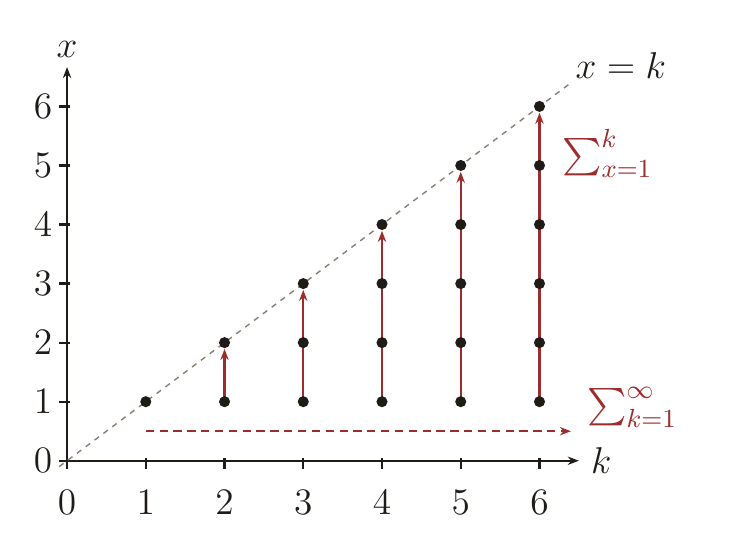
\begin{tikzpicture}[
  x=1cm,
  y=1cm,
  every node/.style={font=\fontsize{13.5}{16}\selectfont, journalink},
  axis/.style={journalink, line width=0.8pt, -{Stealth[length=4pt]}},
  tick/.style={journalink, line width=0.8pt},
  guide/.style={journalmuted, line width=0.5pt, dash pattern=on 2pt off 2pt},
  innersum/.style={journalaccent, line width=0.8pt, -{Stealth[length=4pt]}},
  outersum/.style={journalaccent, line width=0.8pt,
                   dash pattern=on 3pt off 2pt, -{Stealth[length=4pt]}},
  gridpt/.style={circle, fill=journalink, inner sep=0pt, minimum size=4pt},
  sumlab/.style={journalaccent, inner sep=0pt}
]
  % ---- common bounding box, identical in both figures of this pair ----
  \path (-0.50,-0.90) rectangle (8.30,5.50);

  % ---- axes ----
  \draw[axis] (0,0) -- (6.5,0);
  \draw[axis] (0,0) -- (0,5);
  \node[anchor=west,  inner sep=0pt] at (6.65,0) {$k$};
  \node[anchor=south, inner sep=0pt] at (0,5.12) {$x$};

  % ---- ticks on the k axis ----
  \foreach \k in {0,1,2,3,4,5,6} {
    \draw[tick] (\k,0.035) -- (\k,-0.106);
    \node[anchor=north] at (\k,-0.25) {$\k$};
  }

  % ---- ticks on the x axis (one integer step of x is 0.75 units) ----
  \foreach \y/\lab in {0.75/1, 1.5/2, 2.25/3, 3/4, 3.75/5, 4.5/6}
    \draw[tick] (0.035,\y) -- (-0.106,\y)
      node[anchor=east, inner sep=2pt] {$\lab$};
  \draw[tick] (0.035,0) -- (-0.106,0) node[anchor=east, inner sep=2pt] {$0$};

  % ---- boundary of the summation region, x = k ----
  \draw[guide] (-0.1,-0.075) -- (6.4,4.8);
  \node[anchor=south west, inner sep=1.5pt] at (6.4,4.8) {$x=k$};

  % ---- inner sum: solid, upwards along x, from x = 1 to x = k ----
  \draw[innersum] (2,0.75) -- (2,1.42);
  \draw[innersum] (3,0.75) -- (3,2.17);
  \draw[innersum] (4,0.75) -- (4,2.92);
  \draw[innersum] (5,0.75) -- (5,3.67);
  \draw[innersum] (6,0.75) -- (6,4.42);
  \node[sumlab, anchor=west] at (6.28,3.9) {$\sum_{x=1}^{k}$};

  % ---- outer sum: dashed, rightwards along k, from k = 1 to infinity ----
  \draw[outersum] (1,0.375) -- (6.4,0.375);
  \node[sumlab, anchor=west] at (6.6,0.68) {$\sum_{k=1}^{\infty}$};

  % ---- the lattice points, all integer pairs with k >= x (drawn last) ----
  \foreach \k in {1,2,3,4,5,6} \node[gridpt] at (\k,0.75) {};
  \foreach \k in {2,3,4,5,6}   \node[gridpt] at (\k,1.5)  {};
  \foreach \k in {3,4,5,6}     \node[gridpt] at (\k,2.25) {};
  \foreach \k in {4,5,6}       \node[gridpt] at (\k,3)    {};
  \foreach \k in {5,6}         \node[gridpt] at (\k,3.75) {};
  \node[gridpt] at (6,4.5) {};
\end{tikzpicture}
\end{document}
